\section{Summary}
The United States presidential election of 2016 was the 58th quadrennial American presidential election, held on Tuesday, November 8, 2016. The Republican ticket of businessman Donald Trump and Indiana Governor Mike Pence defeated the Democratic ticket of former Secretary of State Hillary Clinton and U.S. Senator from Virginia Tim Kaine. Trump is scheduled to take office as the 45th President, and Pence as the 48th Vice President, on January 20, 2017.

Voters selected members of the Electoral College in each state, in most cases by "winner-takes-all" plurality; those state electors in turn voted for a new president and vice president on December 19, 2016. Leading up to the election, a Trump victory had been considered unlikely by most media forecasts. While Clinton received about 2.9 million more votes nationwide, a margin of 2.1\% of the total cast, Trump won a decisive victory in the Electoral College, winning 30 states with 306 pledged electors out of 538. Trump did so by overturning the perennial swing states of Florida, Iowa and Ohio (the latter two by large margins), as well as the "blue wall" of Michigan, Pennsylvania and Wisconsin, which had been Democratic strongholds to varying degrees since the 1990s.

In the Electoral College vote on December 19, seven electors voted against their pledged candidates: two against Trump and five against Clinton. A further three electors attempted to vote against Clinton but were replaced or forced to vote again. Ultimately, Trump received 304 electoral votes and Clinton garnered 227, while Colin Powell won three, and John Kasich, Ron Paul, Bernie Sanders, and Faith Spotted Eagle each received one.

Trump will be the fifth person in U.S. history to become president despite losing the nationwide popular vote. He will be the first president without any prior experience in public service, while Clinton was the first woman to be the presidential nominee of a major American party.

\section{Background}
The President and Vice President of the United States must be natural-born citizens of the United States, at least 35 years old, and residents of the United States for a period of at least 14 years. Candidates for the presidency typically seek the nomination of one of the political parties of the United States, in which case each party devises a method (such as a primary election) to choose the candidate the party deems best suited to run for the position. Traditionally, the primary elections are indirect elections where voters cast ballots for a slate of party delegates pledged to a particular candidate. The party's delegates then officially nominate a candidate to run on the party's behalf. The general election in November is also an indirect election, where voters cast ballots for a slate of members of the Electoral College; these electors in turn directly elect the President and Vice President.

President Barack Obama, a Democrat and former U.S. Senator from Illinois, was ineligible to seek reelection to a third term due to restrictions of the Twenty-second Amendment; in accordance with Section I of the Twentieth Amendment, his second term expires at noon on January 20, 2017.

\newpage

\section{Election process}
The series of presidential primary elections and caucuses took place between February and June 2016, staggered among the 50 states, the District of Columbia and U.S. territories. This nominating process was also an indirect election, where voters cast ballots for a slate of delegates to a political party's nominating convention, who in turn elected their party's presidential nominee.

Speculation about the 2016 campaign began almost immediately following the 2012 campaign, with New York magazine declaring the race had begun in an article published on November 8, two days after the 2012 election. On the same day, Politico released an article predicting the 2016 general election would be between Clinton and former Florida Governor Jeb Bush, while a New York Times article named New Jersey Governor Chris Christie and Senator Cory Booker from New Jersey as potential candidates.

\section{Republican Party}

With seventeen major candidates entering the race, starting with Ted Cruz on March 23, 2015, this was the largest presidential primary field for any political party in American history.

Prior to the Iowa caucuses on February 1, 2016, Perry, Walker, Jindal, Graham and Pataki withdrew due to low polling numbers. Despite leading many polls in Iowa, Trump came in second to Cruz, after which Huckabee, Paul and Santorum withdrew due to poor performances at the ballot box. Following a sizable victory for Trump in the New Hampshire primary, Christie, Fiorina and Gilmore abandoned the race. Bush followed suit after scoring fourth place to Trump, Rubio and Cruz in South Carolina. On March 1, 2016, the first of four "Super Tuesday" primaries, Rubio won his first contest in Minnesota, Cruz won Alaska, Oklahoma and his home of Texas and Trump won the other seven states that voted. Failing to gain traction, Carson suspended his campaign a few days later. On March 15, 2016, the second "Super Tuesday", Kasich won his only contest in his home state of Ohio and Trump won five primaries including Florida. Rubio suspended his campaign after losing his home state.

Between March 16 and May 3, 2016, only three candidates remained in the race: Trump, Cruz and Kasich. Cruz won most delegates in four Western contests and in Wisconsin, keeping a credible path to denying Trump the nomination on first ballot with 1,237 delegates. Trump then augmented his lead by scoring landslide victories in New York and five Northeastern states in April, followed by a decisive victory in Indiana on May 3, 2016, securing all 57 of the state's delegates. Without any further chances of forcing a contested convention, both Cruz and Kasich suspended their campaigns. Trump remained the only active candidate and was declared the presumptive Republican nominee by Republican National Committee chairman Reince Priebus on the evening of May 3, 2016.

\begin{figure}[!h]
	\begin{center}
		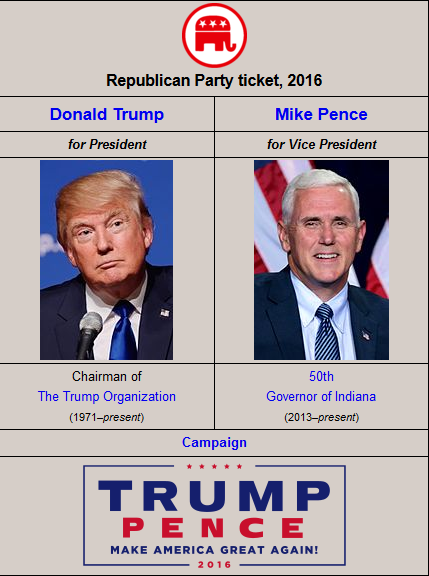
\includegraphics[width=0.6\linewidth]{images/trump}
		\caption{Logo and picture of Trump and Fence}
	\end{center}
\end{figure}

\newpage


\section{Democratic Party}

Former Secretary of State Hillary Clinton, who also served in the U.S. Senate and was the First Lady of the United States, became the first Democrat to formally launch a major candidacy for the presidency. Clinton made the announcement on April 12, 2015, via a video message. While nationwide opinion polls in 2015 indicated that Clinton was the front-runner for the 2016 Democratic presidential nomination, she faced challenges from Independent Senator Bernie Sanders of Vermont, who became the second major candidate when he formally announced on April 30, 2015, that he was running for the Democratic nomination. September 2015 polling numbers indicated a narrowing gap between Clinton and Sanders. On May 30, 2015, former Governor of Maryland Martin O'Malley was the third major candidate to enter the Democratic primary race, followed by former Independent Governor and Republican Senator of Rhode Island Lincoln Chafee on June 3, 2015, former Virginia Senator Jim Webb on July 2, 2015, and former Harvard law professor Lawrence Lessig on September 6, 2015.

\begin{figure}[!h]
	\begin{center}
		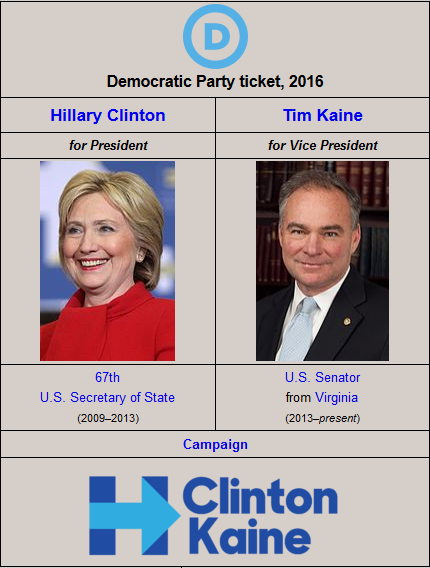
\includegraphics[width=0.6\linewidth]{images/clinton}
		\caption{Logo and picture of Clinton and Kaine}
	\end{center}
\end{figure}

\newpage

\section{Third parties and independents}

Third party and independent candidates that have obtained more than 100,000 votes nationally and one percent of the vote in at least one state, are listed separately.

	\subsection{Libertarian Party}
	Gary Johnson, 29th Governor of New Mexico. Vice-presidential nominee: Bill Weld, 68th Governor of Massachusetts.
	
	\subsection{Green Party}
	Jill Stein, Physician from Lexington, Massachusetts. Vice-presidental nominee: Ajamu Baraka, Acitivist from Washington.
	
	\subsection{Independents}
	Evan McMullin, Chief policy director for the House Republican Conference. Vice-presidential nominee: Mindy Finn, President of Empowered Women.
	
	\subsection{Constitution Party}
	Darrel Castle, Attorney from Memphis, Tennesse. Vice-presidential nominee: Scott Bradley, Businessman from Utah
\section{General election campaign}

	% Please add the following required packages to your document preamble:
	% \usepackage[normalem]{ulem}
	% \useunder{\uline}{\ul}{}
	\begin{table}[!h]
		\centering
		\caption{Money raised per Candidate}
		\label{money}
		\begin{tabular}{|l|l|l|l|l|}
			\hline
			\textbf{Candidate}       & \multicolumn{4}{l|}{\textbf{Campaign committee}}                          \\ \hline
			& {\ul Money raised} & {\ul Money spent} & {\ul Cash on Hand} & {\ul Debt}  \\ \hline
			\textbf{Hillary Clinton} & \$497,808,791      & \$435,367,811     & \$62,440,979       & \$111,238   \\ \hline
			\textbf{Donal Trump}     & \$247,541,449      & \$231,546,996     & \$15,994,454       & \$2,056,572 \\ \hline
		\end{tabular}
	\end{table}

	\subsection{Donald Trump}
	Trump’s candidacy for the Republican nomination in 2016 was initially seen as something of a long shot, but the New York businessman’s outsider status, mastery of the media, and no-holds-barred campaign style propelled him to the front of the field. Trump racked up victories in key early states, and by May the race had dwindled from more than a dozen candidates to three: Trump, Texas Senator Ted Cruz, and Ohio Governor John Kasich. After a critical victory in Indiana on May 3, Cruz and Kasich dropped out, leaving Trump unchallenged for the nomination. When the dust settled, 13.3 million primary voters had backed Trump, a new record in the history of Republican primaries. 
	
	\begin{itemize}
		\item Trump's slogan throughout his campaign was "Make America Great Again," which Trump defined in his book, Crippled America, as "restoring a sense of dignity to the White House, and to our country in general."
		
		\item States that were critical to Trump's victory in the primaries include New Hampshire, Nevada, Florida, New York, and Indiana. 
		
		\item Focal points of Trump's campaign included strengthening U.S. immigration laws, renegotiating or withdrawing from international trade deals, a more aggressive foreign policy in the Middle East, lowering taxes, and repealing financial and environmental regulations.
	\end{itemize}


	\subsection{Hilary Clinton}
	Clinton launched her first presidential campaign on January 20, 2007. In the early months of the Democratic primary, she led then-Sens. Barack Obama and John Edwards in national polls, but was narrowly defeated by Obama after key losses in states like Iowa and North Carolina. In her concession speech on June 8, 2008, Clinton noted the historic nature of her performance, "Although we were not able to shatter that highest and hardest glass ceiling this time, thanks to you it has 18 million cracks in it."
	
	A month after Obama won the general election, he announced that Clinton would serve in his cabinet as secretary of state. While acting as the nation's top diplomat from 2009 to 2013, Clinton used a private email server to conduct official state business, raising questions about her compliance with government regulations on record-keeping and security that have followed her throughout her second presidential run.
	
	Clinton formally received the Democratic Party's presidential nomination on July 26, 2016, after defeating U.S. Sen. Bernie Sanders in a closely contested primary. In doing so, she became the first woman to be nominated for president by a major political party in the United States. 
	
	\begin{itemize}
		\item Clinton served as U.S. senator from New York from 2001 to 2009 and secretary of state from 2009 to 2013.
		
		\item Clinton previously ran for president in 2008. She was defeated by Barack Obama in the Democratic primary by less than one percentage point in the popular vote.
		
		\item Clinton described herself as "a progressive who likes to get things done" and emphasized working across party lines to achieve policy change.
	\end{itemize}
	
\newpage
	
\section{Results 2016}
The election was held on November 8, 2016. Democratic candidate Hillary Clinton cast her vote in the New York City suburb of Chappaqua, while Republican candidate Donald Trump voted in a Manhattan public school. Throughout the day, the election process went more smoothly than many had expected, with only a few reports of long lines and equipment problems.

\begin{table}[!h]
	\centering
	\caption{Results of election, Top candidates}
	\label{result}
	\begin{tabular}{|l|l|l|l|l|}
		\hline
		\textbf{Presidential candidate} & \textbf{Party} & \textbf{Home state} & \textbf{Popular vote} & \textbf{Electoral vote} \\ \hline
		\textbf{Donal Trump}            & Republican     & New York            & 62,979,879; 45,95\%   & 304                     \\ \hline
		\textbf{Hillary Clinton}        & Democratic     & New York            & 65,844,954; 48,04\%   & 227                     \\ \hline
	\end{tabular}
\end{table}

\begin{figure}[!h]
	\begin{center}
		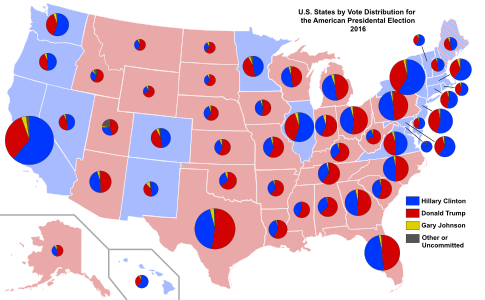
\includegraphics[width=0.8\linewidth]{images/map}
		\caption{Result map of the United States}
	\end{center}
\end{figure}


